\section{Experiments}
\label{sec:experiments}

Our experiments address five questions:
\textbf{Q1:} Does OSTRA outperform baseline policies across simulation
benchmarks (\cref{sec:simulation_experiments})?
\textbf{Q2:} Do these benefits hold in real-world manipulation
(\cref{sec:real_world_experiments})?
\textbf{Q3:} How do errors and computational costs in the foundation-model
components affect OSTRA? We study their impact on task success in
\cref{sec:system_error_breakdown} and their latency in \cref{sec:latency}.
\textbf{Q4:} Which architectural designs contribute to performance?
\textbf{Q5:} How sensitive is OSTRA to its key hyperparameters?
The last two questions are addressed by the design ablations and
hyperparameter analysis in \cref{sec:ablation_studies}.

\begin{figure}[t]
    \centering
    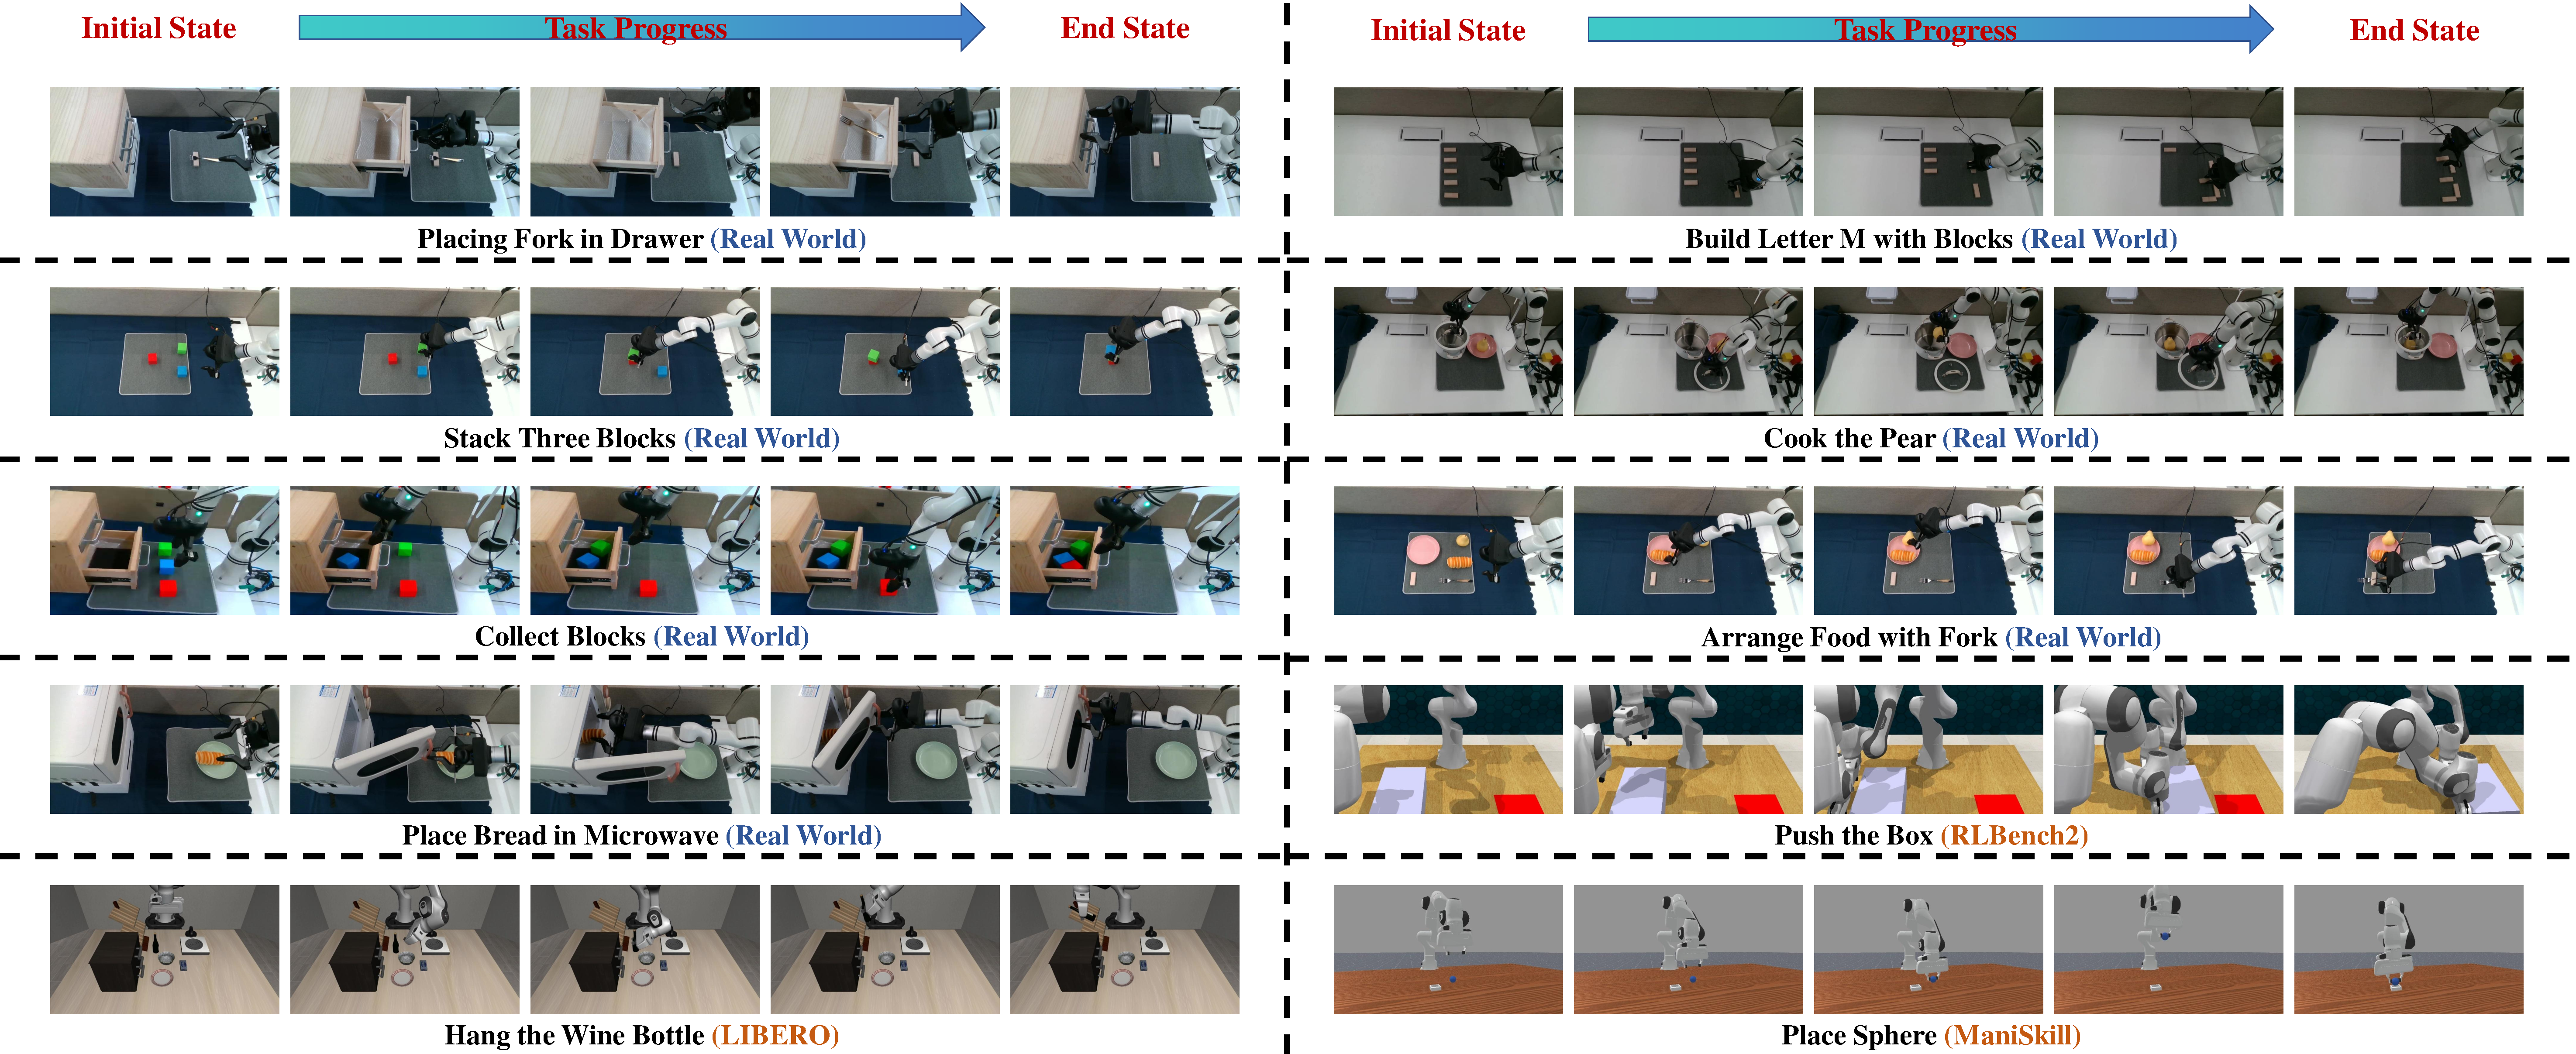
\includegraphics[width=\textwidth]{fig/4_demonstration.pdf}
    \vspace{-20pt}
    \caption{Task demonstrations from initial state to task completion.
    The seven real-world tasks are \textit{Place Fork in Drawer},
    \textit{Stack Three Blocks}, \textit{Collect Blocks},
    \textit{Place Bread in Microwave}, \textit{Build Letter M with Blocks},
    \textit{Cook the Pear}, and \textit{Arrange Food with Fork}.
    The figure also shows representative tasks from the three simulation
    benchmarks: \textit{Push the Box} from
    RLBench2~\citep{James2020RLBench}, \textit{Place Sphere} from
    ManiSkill~\citep{Gu2023ManiSkill2}, and \textit{Hang the Wine Bottle}
    from LIBERO~\citep{liu2023libero}, together spanning articulated,
    contact-rich, and long-horizon robot manipulation challenges.}
    \label{fig:demonstration}
    \vspace{-12pt}
\end{figure}

\begin{table*}[t]
    % \vspace{-6pt}
    \centering
    \caption{\textbf{Real-world manipulation results.}
    We report full-task success rate (\%) over 20 trials per task and the
    average across seven tasks. \textbf{Bold} and \underline{underlining}
    denote the best and second-best results, respectively, using identical
    trial counts for every policy in the matched comparison.}
    \label{tab:real_world_results}
    \vspace{2pt}
    \scriptsize
    \setlength{\tabcolsep}{4pt}
    \resizebox{\textwidth}{!}{%
    \begin{tabular}{lcccccccc}
        \toprule
        \rowcolor{tablehead}
        Method
        & Avg. $\uparrow$
        & \shortstack{Place Fork\\in Drawer}
        & \shortstack{Stack Three\\Blocks}
        & \shortstack{Arrange Food\\with Fork}
        & \shortstack{Place Bread\\in Microwave}
        & \shortstack{Build Letter M\\with Blocks}
        & \shortstack{Collect\\Blocks}
        & \shortstack{Cook the\\Pear} \\
        \midrule
        ACT~\citep{Zhao2023Learning}                    & 19.3 & 15 & 10 & 35 & 20 &  0 & 30 & 25 \\
        Diffusion Policy~\citep{chi2024diffusionpolicy} & 20.0 & 10 &  5 & 40 & 20 &  0 & 35 & 30 \\
        DP3~\citep{Ze2024DP3}                           & 40.7 & 40 & 20 & 65 & 45 &  0 & 60 & 55 \\
        PPI~\citep{Yang2025PPI}                         & 50.7 & 50 & 30 & 75 & 55 & 10 & 70 & 65 \\
        SAM2Act+~\citep{Fang2025SAM2Act}                & \underline{59.3} & \underline{55} & \underline{40} & \underline{85} & \underline{65} & \underline{15} & \underline{80} & \underline{75} \\
        MemoryVLA~\citep{shi2025memoryvla}              & 54.3 & 50 & 35 & 80 & 60 & 10 & 75 & 70 \\
        MPI~\citep{Zeng2024MPI}                         & 44.3 & 45 & 25 & 70 & 50 &  0 & 65 & 55 \\
        SPOT~\citep{Hsu2025SPOT}                        & 52.1 & 45 & 35 & 80 & 55 & 10 & 75 & 65 \\
        Im2Flow2Act~\citep{xu2024im2flow2act}           & 42.9 & 40 & 25 & 70 & 45 &  5 & 60 & 55 \\
        \midrule
        \rowcolor{tablehead} 
        OSTRA (Ours)                                    & \textbf{84.3} & \textbf{85} & \textbf{80} & \textbf{95} & \textbf{85} & \textbf{65} & \textbf{90} & \textbf{90} \\
        \bottomrule
    \end{tabular}%
    }
    \vspace{-6pt}
\end{table*}


\begin{table}[t]
\vspace{-6pt}
\centering
\caption{System error breakdown for OSTRA. We use ground-truth replacements to
identify the dominant bottleneck in OST-Map construction. Ground-truth quantities
are used only for analysis and are not part of the inference interface.
$\Delta$ reports the improvement over Full OSTRA.}
\label{tab:system_breakdown}
\vspace{2pt}
\small
\setlength{\tabcolsep}{6pt}
\begin{adjustbox}{max width=0.9\columnwidth}
\begin{tabular}{l|ccc|>{\columncolor{white}}c|c}
\toprule
Setting & GT Extraction & GT Object Pose & GT Structural Size & Avg. Success & $\Delta$ \\
\midrule
Full OSTRA & & & & \cellcolor{blue1}89.8 & 0.0 \\
+ GT Extraction & $\checkmark$ & & & \cellcolor{blue1}90.3 & +0.5 \\
+ GT Object Pose & & $\checkmark$ & & \cellcolor{blue2}91.9 & +2.1 \\
+ GT Structural Size & & & $\checkmark$ & \cellcolor{blue2}93.4 & +3.6 \\
+ GT Extraction + GT Object Pose & $\checkmark$ & $\checkmark$ & &
\cellcolor{blue2}92.1 & +2.3 \\
+ GT Extraction + GT Structural Size & $\checkmark$ & & $\checkmark$ &
\cellcolor{blue3}94.2 & +4.4 \\
+ GT Object Pose + GT Structural Size & & $\checkmark$ & $\checkmark$ &
\cellcolor{blue4}95.7 & +5.9 \\
+ GT Extraction + GT Object Pose + GT Structural Size
& $\checkmark$ & $\checkmark$ & $\checkmark$
& \cellcolor{blue4}96.4 & +6.6 \\
\bottomrule
\end{tabular}
\end{adjustbox}
\vspace{-8pt}
\end{table}


\begin{table}[t]
    % \vspace{-6pt}
    \centering
    \caption{\textbf{Inference latency (ms) and throughput.}
    We report mean component and end-to-end latency for the first frame and
    subsequent frames at batch size one. The first frame initializes OST-Map.
    Subsequent frames track objects and update the map for end-to-end comparison.}
    \label{tab:latency}
    \vspace{2pt}
    \footnotesize
    \renewcommand{\arraystretch}{1.22}
    \setlength{\tabcolsep}{2pt}
    \begin{adjustbox}{max width=1.0\columnwidth}
    \begin{tabular}{lcccccc}
        \toprule
        \rowcolor{tablehead}
        Stage
        & Mask Seg. / Track. $\downarrow$
        & Pose Reg. / Track. $\downarrow$
        & Structure \& Map $\downarrow$
        & Encoders \& Policy $\downarrow$
        & Total (ms) $\downarrow$
        & FPS $\uparrow$ \\
        \midrule
        First Frame (Initialization)
        & 1412.350 & 1386.425 & 21.340 & 15.210 & \cellcolor{blue1}2835.325 & 0.353 \\
        \addlinespace[3pt]
        Later Frames (Tracking)
        & 94.832 & 96.155 & 20.125 & 15.180 & \cellcolor{blue1}226.292 & 4.419 \\
        \bottomrule
    \end{tabular}
    \end{adjustbox}
    % Feature/map encoding includes DINO, Semantic Field, and OST-Map encoding.
    % Policy timing includes the complete denoising loop. Map update includes
    % first-frame initialization and only invoked operations on later frames.
    % FPS = 1000 / end-to-end latency in ms for sequential processing,
    % not the robot control frequency. -- denotes an unmeasured value.
    \vspace{-6pt}
\end{table}


\begin{table*}[t]
    \vspace{-6pt}
    \centering
    \begin{minipage}[t]{0.5185\textwidth}
    \centering
    \caption{\textbf{OST-Map ablations on RLBench2.}
    We vary temporal supervision and map attributes under a fixed graph encoder.
    Ex11 is OSTRA.}
    \label{tab:ablation_transition_design}
    \vspace{2pt}
    \scriptsize
    \renewcommand{\arraystretch}{1.12}
    \setlength{\tabcolsep}{2pt}
    \raisebox{-\height}{\resizebox{\linewidth}{!}{%
    \begin{tabular}{c|cc|cccc|cccc|c}
        \toprule
        \rowcolor{tablehead}
        & \multicolumn{2}{c|}{Temporal}
        & \multicolumn{4}{c|}{Node}
        & \multicolumn{4}{c|}{Edge}
        & \\
        \rowcolor{tablehead}
        & Hist. & Fut.
        & Geo & Pose & Sem & Aff
        & Type & Param & Anchor & RelPose
        & \textbf{Mean} \\
        \midrule
        Ex1 & -- & --
        & -- & -- & -- & -- & -- & -- & -- & --
        & \cellcolor{blue1}69.4 \\
        Ex2 & $\checkmark$ & --
        & $\checkmark$ & $\checkmark$ & $\checkmark$ & $\checkmark$
        & $\checkmark$ & $\checkmark$ & $\checkmark$ & $\checkmark$
        & \cellcolor{blue3}84.5 \\
        Ex3 & -- & $\checkmark$
        & $\checkmark$ & $\checkmark$ & $\checkmark$ & $\checkmark$
        & $\checkmark$ & $\checkmark$ & $\checkmark$ & $\checkmark$
        & \cellcolor{blue3}85.8 \\
        \midrule
        Ex4 & $\checkmark$ & $\checkmark$
        & -- & $\checkmark$ & -- & -- & -- & -- & -- & --
        & \cellcolor{blue1}75.1 \\
        Ex5 & $\checkmark$ & $\checkmark$
        & $\checkmark$ & $\checkmark$ & -- & -- & -- & -- & -- & --
        & \cellcolor{blue2}78.8 \\
        Ex6 & $\checkmark$ & $\checkmark$
        & $\checkmark$ & $\checkmark$ & $\checkmark$ & --
        & -- & -- & -- & --
        & \cellcolor{blue2}82.5 \\
        Ex7 & $\checkmark$ & $\checkmark$
        & $\checkmark$ & $\checkmark$ & $\checkmark$ & $\checkmark$
        & -- & -- & -- & --
        & \cellcolor{blue3}85.2 \\
        \midrule
        Ex8 & $\checkmark$ & $\checkmark$
        & $\checkmark$ & $\checkmark$ & $\checkmark$ & $\checkmark$
        & $\checkmark$ & -- & -- & --
        & \cellcolor{blue3}86.6 \\
        Ex9 & $\checkmark$ & $\checkmark$
        & $\checkmark$ & $\checkmark$ & $\checkmark$ & $\checkmark$
        & $\checkmark$ & $\checkmark$ & -- & --
        & \cellcolor{blue4}87.8 \\
        Ex10 & $\checkmark$ & $\checkmark$
        & $\checkmark$ & $\checkmark$ & $\checkmark$ & $\checkmark$
        & $\checkmark$ & $\checkmark$ & $\checkmark$ & --
        & \cellcolor{blue4}88.9 \\
        \rowcolor{tablehead}
        \textbf{Ex11} & $\checkmark$ & $\checkmark$
        & $\checkmark$ & $\checkmark$ & $\checkmark$ & $\checkmark$
        & $\checkmark$ & $\checkmark$ & $\checkmark$ & $\checkmark$
        & \cellcolor{blue4}\textbf{89.8} \\
        \bottomrule
    \end{tabular}%
    }}
\end{minipage}
%
    \hfill
    \begin{minipage}[t]{0.4615\textwidth}
    \centering
    \caption{\textbf{OSTRA ablations on RLBench2.}
    We vary attention order, prediction stages, and stop-gradient boundaries.
    Ex12 is OSTRA.}
    \label{tab:ablation_architecture}
    \vspace{2pt}
    \scriptsize
    \renewcommand{\arraystretch}{1.12}
    \setlength{\tabcolsep}{2pt}
    \raisebox{-\height}{\resizebox{\linewidth}{!}{%
    \begin{tabular}{c|cccc|ccc|cc|c}
        \toprule
        \rowcolor{tablehead}
        & \multicolumn{4}{c|}{Attention}
        & \multicolumn{3}{c|}{Denoising}
        & \multicolumn{2}{c|}{Stop-Grad.} & \\
        \rowcolor{tablehead}
        & Map & Vis. & $M\!\to\!V$ & $V\!\to\!M$
        & Obj. & TCP & Hier. & Obj. & TCP & \textbf{Mean} \\
        \midrule
        Ex1 & $\checkmark$ & -- & -- & --
        & $\checkmark$ & $\checkmark$ & $\checkmark$
        & $\checkmark$ & $\checkmark$ & \cellcolor{blue1}76.5 \\
        Ex2 & -- & $\checkmark$ & -- & --
        & $\checkmark$ & $\checkmark$ & $\checkmark$
        & $\checkmark$ & $\checkmark$ & \cellcolor{blue2}78.2 \\
        Ex3 & $\checkmark$ & $\checkmark$ & -- & --
        & $\checkmark$ & $\checkmark$ & $\checkmark$
        & $\checkmark$ & $\checkmark$ & \cellcolor{blue3}85.4 \\
        Ex4 & $\checkmark$ & $\checkmark$ & -- & $\checkmark$
        & $\checkmark$ & $\checkmark$ & $\checkmark$
        & $\checkmark$ & $\checkmark$ & \cellcolor{blue4}87.1 \\
        \midrule
        Ex5 & $\checkmark$ & $\checkmark$ & $\checkmark$ & --
        & -- & -- & -- & -- & -- & \cellcolor{blue1}75.8 \\
        Ex6 & $\checkmark$ & $\checkmark$ & $\checkmark$ & --
        & $\checkmark$ & -- & $\checkmark$
        & $\checkmark$ & -- & \cellcolor{blue2}83.4 \\
        Ex7 & $\checkmark$ & $\checkmark$ & $\checkmark$ & --
        & -- & $\checkmark$ & $\checkmark$
        & -- & $\checkmark$ & \cellcolor{blue3}84.6 \\
        Ex8 & $\checkmark$ & $\checkmark$ & $\checkmark$ & --
        & $\checkmark$ & $\checkmark$ & --
        & -- & -- & \cellcolor{blue2}81.5 \\
        \midrule
        Ex9 & $\checkmark$ & $\checkmark$ & $\checkmark$ & --
        & $\checkmark$ & $\checkmark$ & $\checkmark$
        & -- & -- & \cellcolor{blue3}85.9 \\
        Ex10 & $\checkmark$ & $\checkmark$ & $\checkmark$ & --
        & $\checkmark$ & $\checkmark$ & $\checkmark$
        & $\checkmark$ & -- & \cellcolor{blue4}87.4 \\
        Ex11 & $\checkmark$ & $\checkmark$ & $\checkmark$ & --
        & $\checkmark$ & $\checkmark$ & $\checkmark$
        & -- & $\checkmark$ & \cellcolor{blue4}88.3 \\
        \rowcolor{tablehead}
        \textbf{Ex12} & $\checkmark$ & $\checkmark$ & $\checkmark$ & --
        & $\checkmark$ & $\checkmark$ & $\checkmark$
        & $\checkmark$ & $\checkmark$ & \cellcolor{blue4}\textbf{89.8} \\
        \bottomrule
    \end{tabular}%
    }}
\end{minipage}
%
    \vspace{-6pt}
\end{table*}


\begin{figure}[t]
    \centering
    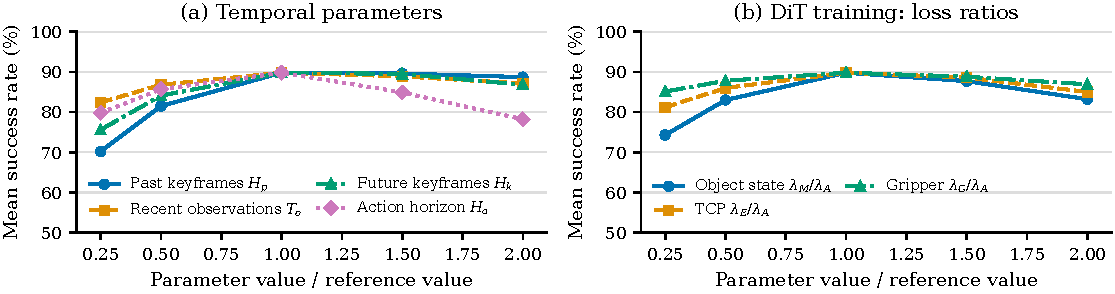
\includegraphics[width=1.0\columnwidth]{fig/6_hyperparameter_sensitivity.pdf}
    \vspace{-20pt}
    \caption{Hyperparameter sensitivity on RLBench2.
    (a) Past keyframes $H_p$, consecutive observations $T_o$, future keyframes
    $H_k$, and predicted actions $H_a$.
    (b) Object-state, TCP, and gripper loss weights relative to the action loss.
    Each curve varies one parameter with all others fixed at their reference
    values. The reference values are $H_p=T_o=H_k=4$, $H_a=16$, and
    $\lambda_M/\lambda_A=\lambda_E/\lambda_A=\lambda_G/\lambda_A=1$.
    All sweeps use the same evaluation protocol.}
    \label{fig:hyperparameter_sensitivity}
    \vspace{-12pt}
\end{figure}

\subsection{Simulation Experiments}
\label{sec:simulation_experiments}

\textbf{Benchmarks and Experimental Setup.}
We benchmark OSTRA on three manipulation suites, with representative task
rollouts shown in \cref{fig:demonstration}.
\textbf{RLBench2}, based on RLBench~\citep{James2020RLBench}, contains seven
multi-stage tasks requiring long-horizon object-state reasoning.
\textbf{ManiSkill}~\citep{Gu2023ManiSkill2} contains six contact-rich insertion,
placement, tool-use, and stacking tasks.
\textbf{LIBERO}~\citep{liu2023libero} contains four ten-task suites---Spatial,
Object, Goal, and Long---for diverse language-conditioned manipulation.
We use benchmark-specific datasets and protocols and report task success rate.
Implementation and benchmark details are provided in
Appendices~\ref{app:implementation_details} and~\ref{app:benchmarks}.


\textbf{Baselines.}
We compare OSTRA with benchmark-specific methods spanning action generation,
history and memory, future prediction, and object-centric perception and
motion~\citep{Zhao2023Learning,chi2024diffusionpolicy,Ze2024DP3,
Fang2025SAM2Act,Yang2025PPI,zhu2023learning,Hsu2025SPOT}.
Detailed descriptions of all baselines are provided in
Appendix~\ref{app:baseline_details}.

\textbf{Simulation results.}
As summarized in \cref{tab:main_results_summary}, OSTRA achieves $89.8\%$,
$74.5\%$, and $97.4\%$ on RLBench2, ManiSkill, and LIBERO, improving over
their strongest reported baselines by $5.3$, $17.7$, and $0.7$ points.
The gains are especially pronounced on representative multi-stage tasks. On
RLBench2, OSTRA reaches $82.7\%$ on Laptop and $77.7\%$ on Handover, improving
over the strongest baselines by $30.7$ and $9.2$ points, respectively. On
ManiSkill, it achieves $79\%$ on Pull Cube with Tool and $50\%$ on Stack
Pyramid, gains of $22$ and $18$ points. These tasks require tool-mediated
interaction, articulated state changes, or sequential object arrangements,
where success depends on reaching appropriate intermediate object states
rather than predicting a single short-horizon motion.
Complete per-task results and method comparisons across benchmarks are reported in
Appendix~\ref{app:full_sim_results}.

\subsection{Real-World Experiments}
\label{sec:real_world_experiments}

We evaluate OSTRA on a 7-DoF Realman 75-BF arm with a Pika parallel gripper.
An Intel RealSense D415 captures RGB-D observations, and
Open3D~\citep{Zhou2018Open3D} reconstructs point clouds. The map constructor
uses predicted masks, poses, and structural parameters, evaluating reasoning
under errors accumulated by the OST-Map perception pipeline. Appendix
~\ref{app:real_world_details} provides the complete hardware, task, and
evaluation protocol.

\textbf{Task suite.}
We consider seven tasks spanning articulated interaction, long-horizon
rearrangement, thin or reflective objects, and global spatial constraints.
They require opening and closing containers, sequential stacking, cluttered
placement, partial-occlusion reasoning, pattern construction, collection, and
shared-workspace manipulation. As visualized in \cref{fig:demonstration}, they
cover articulated state, support, containment, occupancy, and multi-object
layout transitions.

\textbf{Real-world results.}
Across 20 trials per task (\cref{tab:real_world_results}), OSTRA averages
$84.3\%$, exceeds SAM2Act+ ($59.3\%$) by $25.0$ points, and ranks first on all
tasks. It is more reliable on drawer and microwave tasks and better preserves
relations in stacking and shape construction than Diffusion
Policy~\citep{chi2024diffusionpolicy} and DP3~\citep{Ze2024DP3}. Its largest
gain is on \textit{Build Letter M with Blocks} ($65\%$ versus $15\%$), supporting
OST-Map reasoning under noisy, partially occluded observations.

\subsection{System Error Breakdown}
\label{sec:system_error_breakdown}

We use ground-truth replacements to identify which OST-Map Constructor errors
most affect task success.
We replace outputs of SAM 3 extraction, FoundationPose estimation and tracking,
and PointNet--MLP structural estimation with ground-truth masks, poses, or
sizes while fixing the policy and evaluation. We test all eight combinations:
none, each single or pairwise replacement, and all GT. Ground truth is used
only for diagnosis. The complete intervention protocol is provided in
Appendix~\ref{app:additional_experiment_details}.
\Cref{tab:system_breakdown} reports average success relative to Full OSTRA.
Single and joint replacements reveal individual and interacting errors. The
Semantic Field encoder and policy remain unchanged, so all-GT residual failures
are not solely due to map construction.

\subsection{Latency}
\label{sec:latency}

We profile batch-one inference on an NVIDIA GeForce RTX 4090. The first frame
segments masks, registers poses, estimates structure, and initializes OST-Map.
later frames track objects and update the map. Both include encoding and policy
inference. Detailed profiling definitions are provided in
Appendix~\ref{app:additional_experiment_details}.
\Cref{tab:latency} reports $2835.325$ ms for initialization and $226.292$ ms
($4.419$ FPS) thereafter, a $12.5\times$ speedup. Segmentation and pose estimation
dominate. Map construction, encoding, and policy inference add little overhead.

\subsection{Ablation Studies}
\label{sec:ablation_studies}

We ablate OST-Map temporal roles and attributes, map--visual attention order,
staged denoising and stop-gradient, and temporal and loss hyperparameters.
All variants use the same RLBench2 data, capacity, budget, and evaluation seeds.
Appendix~\ref{app:additional_experiment_details} provides the complete
ablation and sensitivity setups used for controlled training, evaluation, and
hyperparameter comparisons in matched settings.

\textbf{OST-Map.}
\Cref{tab:ablation_transition_design} compares no map or future loss (Ex1),
history only (Ex2), future supervision from the latest map (Ex3), and the full
model (Ex11). Ex4--Ex11 progressively add geometry, semantics, affordances,
and edge attributes to pose-only nodes under the same graph encoder and node
correspondence. Full OST-Map reaches $89.8\%$, $20.4$ points above no map.
history-only and future-only reach $84.5\%$ and $85.8\%$. Their combination and
the Ex4--Ex11 trend show that both temporal roles and attribute groups help.

\textbf{Transition-Guided Attention.}
Ex1--Ex4 in \cref{tab:ablation_architecture} test map-only, visual-only, joint,
and visual-first attention against map-first (Ex12), with the full hierarchy
and stop-gradient boundaries. Map-first reaches $89.8\%$, exceeding these
variants by $13.3$, $11.6$, $4.4$, and $2.7$ points, respectively.

\textbf{Staged Denoising.}
With map-first attention fixed, Ex5--Ex8 test action-only, object-to-action,
TCP-to-action, and flat joint prediction. Ex9--Ex12 test object/TCP
stop-gradient combinations. Removed stages omit their heads and losses, while
the flat variant retains all targets without hierarchical conditioning. The
full hierarchy exceeds action-only by $14.0$ points and flat prediction by
$8.3$ points. Both stop-gradient boundaries add $3.9$ points over neither.

\textbf{Hyperparameter sensitivity.}
\Cref{fig:hyperparameter_sensitivity} varies four temporal counts---past
keyframes $H_p$, observations $T_o$, future keyframes $H_k$, and actions
$H_a$---and three loss ratios:
$\lambda_M/\lambda_A$, $\lambda_E/\lambda_A$, and $\lambda_G/\lambda_A$.
Each curve varies one parameter around the $89.8\%$ full-model reference.
Performance is stable nearby but falls at short or long horizons. $H_a$, $H_p$,
and object-state loss are most sensitive, while gripper loss remains stable
across the evaluated range and is less sensitive to its weighting.
